% 06_phase1.tex — owned by the phase1 writer. Numbers: paper/FACTS.md §1, §3, §7, §8 only.
\section{Strategy or frozen learning?}\label{sec:phase1}

Section~\ref{sec:results} ends with a puzzle. The memory-0 learner cannot condition on the past, so it cannot punish, yet it freezes at $\Dl = 0.943$, above the full learner's $0.621$, and the temptation test of Section~\ref{sec:indicators} fires for it all the same, while the ablation reads it as the higher-priced learner. The natural guess is that its high price is an accident of the exploration schedule: $\varepsilon_t$ died before an undercutting race could finish, and the tables froze with stale estimates of what an undercut is worth. This section tests that guess. Five experiments were designed, and their predictions written down, before any of them ran. Each cell uses 100 seeds and the hyperparameters of Section~\ref{sec:design}; each experiment changes one element of the design and, where the change forces it, the horizon or the quantity measured, as stated in its subsection. Table~\ref{tab:predictions} lists the predictions and the outcomes. Two of the five failed outright, two held only in part, and one held with a caveat (Table~\ref{tab:predictions}). The failures are the useful part: a ten-fold longer decay and a change to pay-as-bid do not remove the memory-0 price, which rules out the two readings we tested, a race cut short by the schedule and an artefact of the uniform-price rule in particular. The tables are stale (Section~\ref{sec:residual}), but the staleness is reproduced rather than accidental. Section~\ref{sec:occupation} offers a reading of why; it is a verbal argument, not a result.

\begin{table}[htbp]
\centering
\caption{Pre-registered predictions and outcomes.}
\label{tab:predictions}
\small
\begin{tabular}{@{}clp{5.6cm}p{4.6cm}@{}}
\toprule
\# & Experiment & Prediction & Held? \\
\midrule
1 & $\beta$ sweep (slower decay) & memory-0 $\Dl$ falls toward 0; memory-1 holds & no \\
2 & $\varepsilon$ re-injection & memory-1 re-converges to the same $\Dl$; memory-0 collapses & half: memory-1 yes; memory-0 also re-converges \\
3 & Bellman residual & memory-0 large (stale); memory-1 small (learned) & yes, with a twist: both stale, consequence differs \\
4 & pay-as-bid & (low, high, high) rest point vanishes; memory-0 $\Dl$ falls a lot & no: $\Dl$ falls 0.10, rest point moves, freeze stays \\
5 & constant-$\varepsilon$ occupation & frozen $\Dl = \lim_{\varepsilon\to 0}$ of the time-average $\Dl$ & memory-0 within 0.01; memory-1 within about 0.02 at one point, from above, and needing about 30$\times$ less noise \\
\bottomrule
\end{tabular}
\par\smallskip
\footnotesize Notes: predictions were fixed before the runs; 100 seeds per cell. Two of the five failed outright, two held only in part, and one held with a caveat.
\end{table}

\subsection{Slower exploration decay}\label{sec:beta}

If the memory-0 freeze is a race cut short, a longer race should finish it. The sweep varies $\beta$ in $\varepsilon_t = e^{-\beta t}$ over two orders of magnitude and sets the horizon to $10/\beta$ plus a 4M-round tail, so every cell reaches $\varepsilon = e^{-10}$ and then gets the same greedy tail. At $\beta = 10^{-6}$ the learners get ten times the exploratory rounds of the specification.

\begin{table}[htbp]
\centering
\caption{Frozen $\Dl$ against the exploration decay rate $\beta$.}
\label{tab:sweep}
\small
\begin{tabular}{@{}lrrrr@{}}
\toprule
$\beta$ & Rounds & Memory 0: $\Dl$ (95\% CI) & Memory 1: $\Dl$ (95\% CI) & Memory 1 converged \\
\midrule
$10^{-6}$ & 14M & 0.949 (0.936--0.962) & 0.721 (0.695--0.746) & 88\% \\
$3\times 10^{-6}$ & 7.3M & 0.940 (0.928--0.952) & 0.636 (0.623--0.649) & 100\% \\
$10^{-5}$ (spec) & 5M & 0.943 (0.931--0.954) & 0.621 (0.612--0.630) & 100\% \\
$3\times 10^{-5}$ & 4.3M & 0.957 (0.946--0.968) & 0.618 (0.610--0.626) & 100\% \\
$10^{-4}$ & 4.1M & 0.949 (0.938--0.961) & 0.593 (0.583--0.603) & 100\% \\
\bottomrule
\end{tabular}
\par\smallskip
\footnotesize Notes: horizon $= 10/\beta + 4$M rounds; 100 seeds per cell; memory-0 converged in 100\% of seeds in every cell.
\end{table}

Table~\ref{tab:sweep} rejects the prediction. Memory-0 is flat between 0.940 and 0.957 across the whole range, with overlapping confidence intervals, and it converges in every seed of every cell. A ten-fold longer race did not finish. Memory-1 does not hold either, so the second half of the prediction also fails: slower decay gives higher frozen prices, from 0.593 at $\beta = 10^{-4}$ to 0.721 at $\beta = 10^{-6}$, where 12\% of seeds had not met the convergence criterion by 14M rounds. Within the range tested, the length of a decaying exploration schedule does not change where the memory-0 learner freezes, and for the memory-1 learner slower decay is associated with a higher frozen price.

\subsection{Re-injecting exploration}\label{sec:reinject}

The second test starts from the converged 5M tables and restarts training with $\varepsilon_t = \varepsilon_0 e^{-\beta t}$, $\beta = 10^{-5}$, for 2M rounds, then freezes and measures $\Dl$ again. A learned equilibrium should re-converge to the same price. A stale-table accident should not survive $\varepsilon_0 = 0.5$, which makes half of all early actions random.

\begin{table}[htbp]
\centering
\caption{Re-injecting exploration into converged tables.}
\label{tab:reinject}
\footnotesize
\setlength{\tabcolsep}{4pt}
\begin{tabular}{@{}lrrrrr@{}}
\toprule
 & & $\Dl$ & Seeds & Lowest 1k-round & Low bidder \\
Source & $\varepsilon_0$ & before $\to$ after & dropping $>0.1$ & mean price & changed \\
\midrule
memory 1 & 0.05 & 0.621 $\to$ 0.622 & 4\% & \eur{38} & --- \\
memory 1 & 0.5 & 0.621 $\to$ 0.621 & 5\% & \eur{38} & --- \\
memory 0 & 0.05 & 0.943 $\to$ 0.945 & 11\% & \eur{37} & 71\% \\
memory 0 & 0.5 & 0.943 $\to$ 0.952 & 10\% & \eur{37} & 70\% \\
\bottomrule
\end{tabular}
\par\smallskip
\footnotesize Notes: 100 converged 5M tables per row; restart with $\varepsilon_t = \varepsilon_0 e^{-\beta t}$, $\beta = 10^{-5}$, 2M rounds, then frozen play. ``Low bidder changed'' is the share of memory-0 seeds in which a different firm holds the low bid after the restart.
\end{table}

Table~\ref{tab:reinject} shows that the mean frozen $\Dl$ of both learners returns to its pre-restart value. At $\varepsilon_0 = 0.5$ the memory-0 tables are scrambled: the lowest 1,000-round mean price during the run is \eur{37}, and in 70\% of seeds a different firm ends as the low bidder. The milder restart at $\varepsilon_0 = 0.05$ disrupts the tables just as much (lowest price \eur{37}, low bidder changed in 71\% of seeds), so the return does not depend on the size of the restart. The process nevertheless returns to a mean $\Dl$ of 0.952, with only 10\% of seeds dropping by more than 0.1, and all 100 seeds end again at a profile of the same (low, high, high) shape.
The estimates left behind are stale (Section~\ref{sec:residual}), but the restart reproduces the same kind of stale configuration with the roles reassigned, so the staleness is not an accident of one schedule; whatever produces it operates again whenever exploration fades. Section~\ref{sec:occupation} offers a reading. The memory-1 learner also re-converges, to 0.621 or 0.622, with 4--5\% of seeds dropping. Both learners re-converge, so robustness to a restart does not separate them.

\subsection{The Bellman residual on the temptation action}\label{sec:residual}

Section~\ref{sec:results} showed that the converged cycles carry an unplayed profitable deviation in every full-learner and memory-0 seed. The question is what the table says about it. For every temptation on the converged cycle (firm $i$, state $s$, played action $a_i$, best unplayed deviation $a_{\mathrm{dev}}$) we compute the one-step target $\text{profit}(a_{\mathrm{dev}}, \text{rivals at their greedy actions}) + \gamma \max_a Q_i(s', a)$ and the residual $\text{target} - Q_i(s, a_{\mathrm{dev}})$, and the same for the played action. A residual near zero means the stored value of the deviation agrees with a one-step backup under the learner's own table; if the learner still declines it, the table values the state reached by deviating poorly, a continuation that may itself be stale (Section~\ref{sec:discussion}). A large residual is what one expects if $a_{\mathrm{dev}}$ has rarely or never been played since the rivals settled, so that its estimate dates from the exploration era. The share reported in Table~\ref{tab:residual} is the fraction of temptations for which the one-step target of the unplayed deviation, computed with the current table, exceeds the stored value of the played action, so that a refreshed estimate of the deviation would rank it above the played action.

\begin{table}[htbp]
\centering
\caption{Bellman residual on the temptation action, converged 5M tables.}
\label{tab:residual}
\footnotesize
\setlength{\tabcolsep}{4pt}
\begin{tabular}{@{}lrrrrr@{}}
\toprule
 & Residual, & Residual on $a_{\mathrm{dev}}$ & Share: one backup & Seeds at & Seeds with \\
Configuration & played & (95\% CI) & prefers $a_{\mathrm{dev}}$ & 0\% / 100\% & $\geq 1$ temptation \\
\midrule
Full (memory 1, $\gamma = 0.95$) & $\approx 0$ & \eur{\num{2708}} (\num{2521}--\num{2894}) & 31\% & 12 / 0 & 100 \\
$\gamma = 0$, memory 1 & $\approx 0$ & \eur{865} (824--907) & 100\% & 0 / 95 & 95 \\
Memory 0, $\gamma = 0.95$ & $\approx 0$ & \eur{\num{6656}} (\num{6093}--\num{7218}) & 100\% & 0 / 100 & 100 \\
\bottomrule
\end{tabular}
\par\smallskip
\footnotesize Notes: residual on the played action is of order $10^{-11}$ for the full learner. The five $\gamma = 0$ seeds without a temptation sit at one-shot Nash profiles and are not counted.
\end{table}

Played actions are Bellman-consistent everywhere, as they must be at a rest point of the update. The deviation estimates are non-zero-residual in every configuration, including the full learner, whose residual on $a_{\mathrm{dev}}$ is \eur{\num{2708}} (a difference of discounted values, so not directly comparable with the \eur{865} of the undiscounted $\gamma = 0$ table). The prediction that the memory-1 residual would be small therefore failed in its literal form. For $\gamma = 0$ and memory 0 a refreshed estimate of the deviation would flip the decision in 100\% of temptations, in every seed: the learner sits on money it has not looked at. For the full learner a refreshed estimate of the deviation would flip the decision in 31\% of temptations. In the other 69\% the value the learner's own table assigns to the state reached by deviating is low enough that a refreshed estimate would leave the deviation unattractive. Under the table's own valuation that is a learned continuation, the thing tacit collusion consists of; the valuation is a one-step backup whose continuation term may itself be stale (Section~\ref{sec:discussion}), and whether it deserves the name is not settled here.

The per-seed distribution is what makes this the discriminating test. Among the 100 full-learner seeds, 12 have a share of exactly 0\%, 71 lie in $(0, 50\%]$, 17 lie in $(50\%, 100\%)$, and none is at 100\%; the highest single seed is 80\%. Every memory-0 seed and every $\gamma = 0$ seed is at exactly 100\%. The two distributions do not overlap. Of the behavioural battery only M3 separates the two learners, and it does so because a one-state table cannot react (Section~\ref{sec:results}); the residual share separates them on what their tables value. The price of the test is that it reads the Q-table. It is a tool for simulated learners, not a screen for real bid data.

\subsection{Pay-as-bid}\label{sec:payasbid}

Under uniform pricing the profile (low, high, high) is a natural rest point for the memory-0 learner: the low bidder sells 60 MW at the high price and has no reason to move, and each high bidder can only discover the gain from a one-rung cut through an exploratory draw. If dispatched firms are paid their own bids instead, the low bidder is no longer paid the high price and should want to move up, so the rest point should vanish and $\Dl$ should fall sharply. The reported price stays the marginal bid, so $\Dl$ is comparable.

\begin{table}[htbp]
\centering
\caption{Pay-as-bid: frozen $\Dl$ and the most common frozen profiles, 5M rounds.}
\label{tab:payasbid}
\small
\begin{tabular}{@{}lrl@{}}
\toprule
Configuration & $\Dl$ (95\% CI) & Most common frozen profiles (seeds) \\
\midrule
memory 0, pay-as-bid & 0.845 (0.819--0.871) & (68,68,68) 16; (94,94,94) 12; (81,81,81) 9; (87,87,87) 8 \\
memory 1, pay-as-bid & 0.689 (0.677--0.701) & (55,55,55) 13; (49,49,55) 9; (61,61,61) 8; (49,49,49) 8 \\
\bottomrule
\end{tabular}
\par\smallskip
\footnotesize Notes: 100 seeds per row, converged 100\%. Profiles are the last-round bids in \eur{}/MWh, rounded; a symmetric tie splits the 100 MW three ways at each firm's own bid.
\end{table}

The rest point did vanish. Table~\ref{tab:payasbid} shows memory-0 freezing at symmetric ties, each firm selling a third of demand at its own bid, rather than at (low, high, high). But it freezes all the same, at $\Dl = 0.845$ against 0.943 under uniform pricing, a fall of 0.10. At every one of those ties each firm could gain by shaving one rung: from \eur{\num{1929}} to \eur{\num{3086}} per round at the tie at 67.86 (a gain of \eur{\num{1157}}), and from \eur{\num{2786}} to \eur{\num{4629}} at 93.57 (a gain of \eur{\num{1843}}), with the ties at 80.71 and 87.14 in between. The auction rule changes where the process stops, not whether it stops. The memory-1 learner freezes at lower ties, mostly symmetric, with bids near 49--61, at $\Dl = 0.689$.

\subsection{The occupation measure under constant exploration}\label{sec:occupation}

The last experiment asks what the freeze is. Exploration is held constant at $\varepsilon$ ($\beta = 0$) for 3M rounds (30M rounds for $\varepsilon = 10^{-4}$), the first third is dropped, and the time-average $\Dl$ of the exploring process is recorded, together with the share of recording blocks whose mean price exceeds \eur{55}. If the frozen price is simply where the exploring process lives, the time average should approach the frozen value as $\varepsilon \to 0$.

\begin{table}[htbp]
\centering
\caption{Time-average $\Dl$ under constant exploration.}
\label{tab:occupation}
\footnotesize
\setlength{\tabcolsep}{4pt}
\begin{tabular}{@{}lrrrr@{}}
\toprule
 & \multicolumn{2}{c}{Memory 0} & \multicolumn{2}{c}{Memory 1} \\
\cmidrule(lr){2-3}\cmidrule(lr){4-5}
$\varepsilon$ & time-avg $\Dl$ (95\% CI) & blocks $> \eur{55}$ & time-avg $\Dl$ (95\% CI) & blocks $> \eur{55}$ \\
\midrule
0.1 & 0.446 (0.446--0.446) & 28\% & 0.336 (0.336--0.336) & 0\% \\
0.03 & 0.645 (0.645--0.645) & 62\% & 0.326 (0.325--0.326) & 0\% \\
0.01 & 0.810 (0.809--0.810) & 84\% & 0.333 (0.329--0.336) & 4\% \\
0.003 & 0.903 (0.902--0.905) & 95\% & 0.408 (0.401--0.415) & 24\% \\
0.001 & 0.934 (0.931--0.937) & 98\% & 0.486 (0.477--0.494) & 48\% \\
0.0001 (30M rounds) & not run & & 0.643 (0.635--0.652) & 94\% \\
$\to 0$ (frozen, Table~\ref{tab:sweep}) & 0.943 & & 0.621 & \\
\bottomrule
\end{tabular}
\par\smallskip
\footnotesize Notes: $\beta = 0$; 3M rounds, first third dropped; 100 seeds per cell; the last row is the frozen value from the specification cell.
\end{table}

\begin{figure}[htbp]
\centering
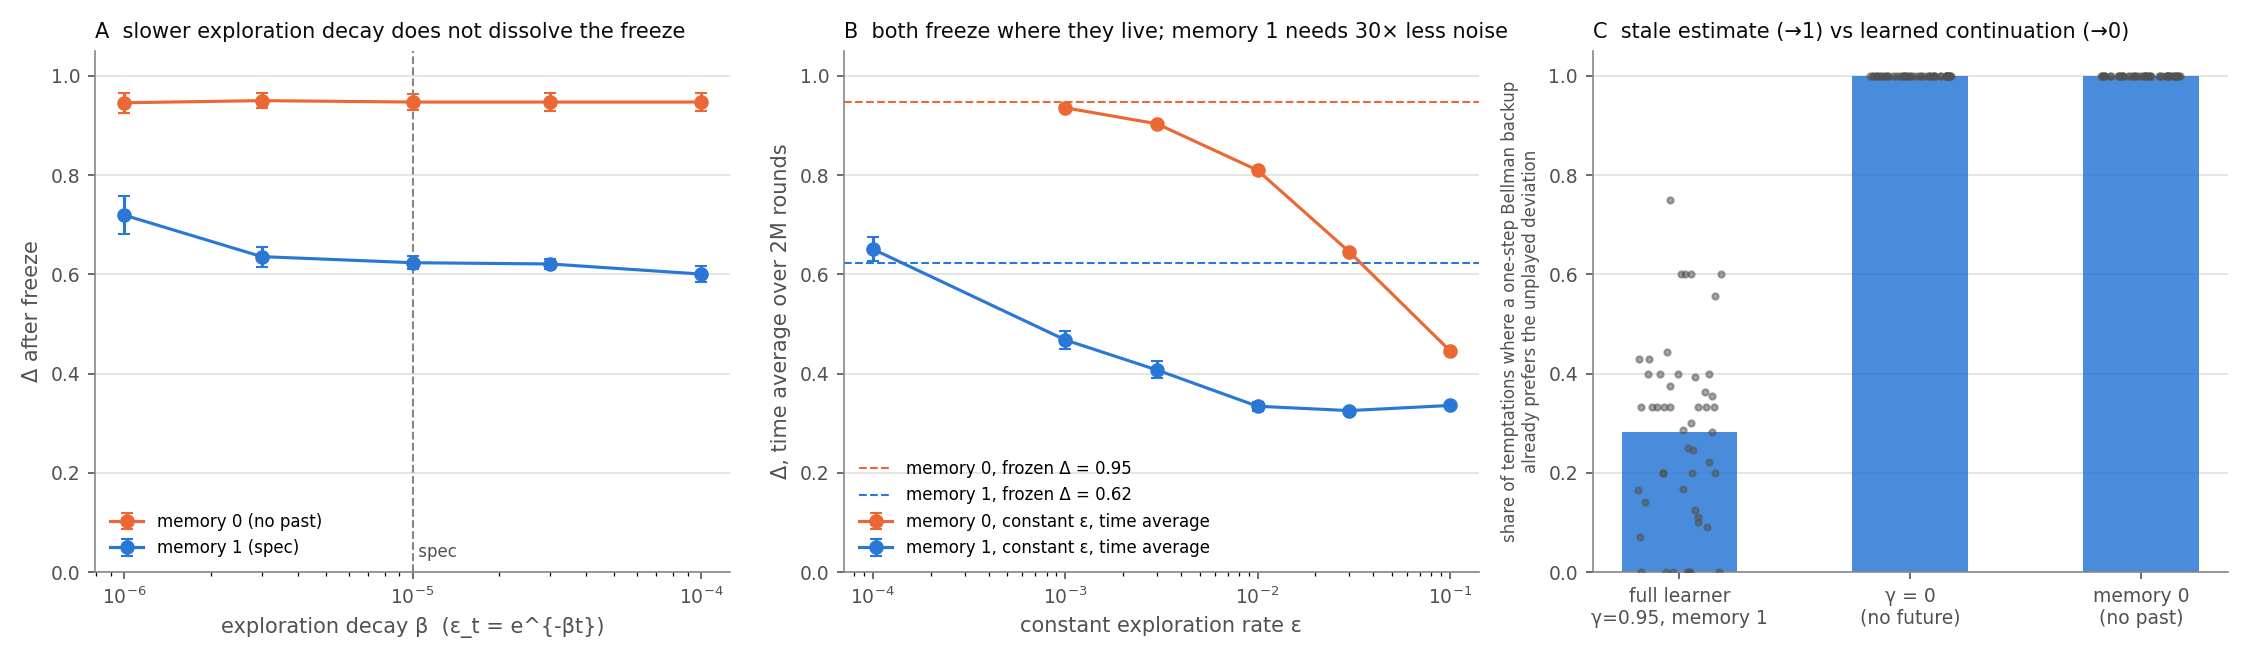
\includegraphics[width=\textwidth]{figures/phase1.png}
\caption{Three views of the Phase 1 evidence. Panel A: frozen $\Dl$ against the decay rate $\beta$ (Table~\ref{tab:sweep}); memory-0 is flat, memory-1 rises as decay slows. Panel B: time-average $\Dl$ under constant $\varepsilon$ (Table~\ref{tab:occupation}) with each learner's frozen value as a dashed line; both curves meet their frozen value as $\varepsilon \to 0$, memory-1 only at $\varepsilon = 10^{-4}$. Panel C: the share of temptations at which one Bellman backup already prefers the unplayed deviation (Table~\ref{tab:residual}), bar = mean, dots = seeds; the full learner sits at 0.31 with no seed at 1, the other two at 1 in every seed.}
\label{fig:phase1}
\end{figure}

Table~\ref{tab:occupation} and Panel B of Figure~\ref{fig:phase1} confirm the prediction for memory-0. The time average rises monotonically as $\varepsilon$ falls and reaches 0.934 at $\varepsilon = 0.001$, within 0.01 of the frozen 0.943; it is already within 5\% at $\varepsilon = 0.003$. The frozen price is the small-noise limit of where the exploring process spends its time. The block-to-block moves are large for memory-0, about \eur{28} in either direction at $\varepsilon \leq 0.03$ (Appendix~\ref{app:extra}), which is consistent with a process that jumps between the top and the bottom of the grid; the block average does not resolve the step-by-step walk down that the argument below assumes, so the asymmetry itself is not observed. 

We read this as a cycle of the Edgeworth type \citep{maskin1988}; what follows is a verbal argument that the experiments are consistent with, not a result, and Section~\ref{sec:discussion} states its limits. An undercut is discovered by an exploratory draw; the firm that is undercut sells less (60 to 40 MW if it was lowest, 20 to 0 if it was one of the tied high bidders), learns this, and undercuts back; the price falls by a rung whenever the second-lowest bid falls. Near the bottom a firm earning nothing loses nothing by raising its bid, and because the price is the second-lowest bid it takes one raise if a rival is already high and two if not; either way each step up is free, whereas each step down needs a specific exploratory draw at a specific time. If so, the exploring process should spend more time near the top the less noise there is, and freezing would sample that distribution; Table~\ref{tab:occupation} is consistent with this and does not test the chain itself. This is a statement about a learning dynamic on a discrete grid, not about strategy. The closest analogy is stochastic stability \citep{kandori1993,young1993}: as the noise vanishes, the states selected are those that take the most rare draws to leave and the fewest to reach, and here the high-price profiles are where the process is found. It is not the folk theorem \citep{fudenberg1986}: there is no threat, and with one state there is no memory to carry one.

The memory-1 learner also meets its frozen value, but far less easily. Its exploring process lives at $\Dl$ between 0.326 and 0.486 for $\varepsilon$ from 0.1 down to 0.001, below its frozen 0.621, and 0\% of blocks exceed \eur{55} for $\varepsilon \geq 0.03$. At $\varepsilon = 0.001$ it is still 0.14 below the frozen value. Only at $\varepsilon = 10^{-4}$, in a 30M-round run, does the time average reach 0.643 and meet it. Memory-0 is within 5\% of its frozen price at $\varepsilon = 0.003$; memory-1 needs roughly 30 times less noise for the same closeness. That is consistent with a coordinated cycle: three agents alternating between a high and a low profile, which any single random draw breaks for a stretch, and which re-forms only when draws are rare. The occupation measure separates the two learners by noise tolerance, not by kind. The Bellman-residual share of Section~\ref{sec:residual} remains the qualitative separator, and Panel C of Figure~\ref{fig:phase1} shows why: the memory-0 and $\gamma = 0$ seeds stack at 1, the full learner's seeds spread below it and none reaches 1. One caveat belongs here. The memory-1 curve has a single point at $\varepsilon = 10^{-4}$, so the location of its transition is not pinned down.

Three things change in the verdict of Section~\ref{sec:results}. The memory-0 price now has a candidate explanation. The experiments are consistent with its being the small-noise limit of an Edgeworth-type cycle run by $\varepsilon$-greedy learners on a discrete grid (a verbal argument, Section~\ref{sec:discussion}); it survives ten-fold slower decay, a restart of exploration from $\varepsilon_0 = 0.5$ that reassigns the low-bidder role in about 70\% of seeds, and a change of auction rule; and on this evidence it is a property of the learning dynamic, not evidence of collusion. The full learner does something the memory-0 learner does not: its deviation estimates are equally stale, but in 69\% of temptations the continuation it has learned is poor enough that a fresh estimate would not change the decision, and under constant exploration its time-average price sits far below its frozen value at noise levels ($\varepsilon \leq 0.003$) at which the memory-0 average is already within 5\% of its own frozen value. The $\Dl$-based ablation was right to fail, because price levels cannot tell these two learners apart, and the one measurement that can, the Bellman-residual share, needs the Q-table.
